\chapter{Experimental Calibration}
\section{Calibration Test Matrices}
{\small
\begin{longtable}{ccc}
\caption{Proposed Test Matrix for Optimal Nozzle height} \label{tab:heightmatrix} \\
\hline
\textbf{Test No.} & \textbf{Nozzle Height (mm)} \\
\hline
\endhead
\hline
1 & 0.2 \\
2 & 0.4 \\
3 & 0.6 \\
4 & 0.8 \\
5 & 1.0 \\
\hline
\end{longtable}
}

{\small
\begin{longtable}{ccc}
\caption{Proposed Test Matrix for Straight Line Experiment} \label{tab:linetestmatrix} \\
\hline
\textbf{Test No.} & \textbf{Printing Speed (mm/s)} & \textbf{Extrusion Speed (mm/s)} \\
\hline
1  & 20 & 0.2 \\
2  & 20 & 0.3 \\
3  & 20 & 0.4 \\
4  & 20 & 0.5 \\
5  & 25 & 0.2 \\
6  & 25 & 0.3 \\
7  & 25 & 0.4 \\
8  & 25 & 0.5 \\
9  & 30 & 0.2 \\
10 & 30 & 0.3 \\
11 & 30 & 0.4 \\
12 & 30 & 0.5 \\
13 & 35 & 0.2 \\
14 & 35 & 0.3 \\
15 & 35 & 0.4 \\
16 & 35 & 0.5 \\
\hline
\end{longtable}
}

{\small
\begin{longtable}{ccc}
\caption{Proposed Test Matrix for Curved Line Experiment} \label{tab:curvetestmatrix} \\
\hline
\textbf{Test No.} & \textbf{Line Radius (mm)} \\
\hline
\endhead
\hline
1  & 5 \\
2  & 15 \\
3  & 25 \\
4  & 35 \\
5  & 45 \\
\hline
\end{longtable}
}
{\small
\begin{longtable}{ccc}
\caption{Proposed Test Matrix for Optimal Spacing of Adjacent Lines} \label{tab:spacingmatrix} \\
\hline
\textbf{Test No.} & \textbf{Line Spacing (mm)} \\
\hline
\endhead
\hline
1 & 3.0 \\
2 & 3.5 \\
3 & 4.0 \\
4 & 4.5 \\
5 & 5.0 \\
6 & 5.5 \\
\hline
\end{longtable}
}
{\small
\begin{longtable}{ccc}
\caption{Proposed Test Matrix for Optimal Layer Stacking Offset} \label{tab:stackingmatrix} \\
\hline
\textbf{Test No.} & \textbf{Layer Offset (mm)} \\
\hline
\endhead
\hline
1 & 1.0 \\
2 & 1.5 \\
3 & 2.0 \\
\hline
\end{longtable}
}
\section{Measured Results}

{\small
\begin{longtable}{>{\raggedright\arraybackslash}p{1cm} 
                  >{\centering\arraybackslash}p{2cm} 
                  >{\centering\arraybackslash}p{2cm} 
                  >{\centering\arraybackslash}p{2cm} 
                  >{\centering\arraybackslash}p{1.5cm} 
                  >{\centering\arraybackslash}p{1.5cm}
                  >{\centering\arraybackslash}p{1.5cm}}
\caption{Calibration Phase 1 - Nozzle Height Test Results}  \label{tab:heightResults} \\
\hline
\textbf{Test No.} & \textbf{Nozzle Height (mm)} & \textbf{Length (mm)} & \textbf{Mean Width (mm)}  & \textbf{Std Dev Width (mm)} \\
\hline
\endhead
\hline
1  & 0.2 & 88 & 2.9 & 0.71 \\
2  & 0.4 & 94 & 3.0 & 0.33 \\
3  & 0.6 & 93 & 3.0 & 0.53 \\
4  & 0.8 & 92 & 3.0 & 0.52 \\
5  & 1.0 & 90 & 2.8 & 0.47 \\
\hline
\end{longtable}
}

{\small
\begin{longtable}{>{\raggedright\arraybackslash}p{1cm} 
                  >{\centering\arraybackslash}p{2cm} 
                  >{\centering\arraybackslash}p{2cm} 
                  >{\centering\arraybackslash}p{2cm} 
                  >{\centering\arraybackslash}p{1.5cm} 
                  >{\centering\arraybackslash}p{2.0cm}}
\caption{Calibration Phase 2 - Straight Line Test Results}  \label{tab:lineResults} \\
\hline
\textbf{Test No.} & \textbf{Print Speed (mm/s)} & \textbf{Extrusion Speed (mm/s)} & \textbf{Length (mm)} & \textbf{Mean Width (mm)}  & \textbf{Std Dev Width (mm)} \\
\hline
\endhead
\hline
1  & 20 & 0.2 &  93 & 3.0 & 0.27 \\
2  & 20 & 0.3 &  94 & 3.6 & 0.57 \\
3  & 20 & 0.4 &  99 & 4.2 & 0.32 \\
4  & 20 & 0.5 & 101 & 4.5 & 0.34 \\
5  & 25 & 0.2 &  85 & 3.2 & 0.46 \\
6  & 25 & 0.3 &  90 & 3.5 & 0.63 \\
7  & 25 & 0.4 &  94 & 3.8 & 0.26 \\
8  & 25 & 0.5 &  98 & 4.1 & 0.56 \\
9  & 30 & 0.2 &  87 & 2.3 & 0.40 \\
10 & 30 & 0.3 &  97 & 2.9 & 0.46 \\
11 & 30 & 0.4 &  98 & 3.7 & 0.45 \\
12 & 30 & 0.5 &  99 & 4.5 & 0.53 \\
13 & 35 & 0.2 &  92 & 2.2 & 0.53 \\
14 & 35 & 0.3 &  95 & 2.9 & 0.74 \\
15 & 35 & 0.4 &  97 & 3.9 & 0.57 \\
16 & 35 & 0.5 &  98 & 4.1 & 0.79 \\
\hline
\end{longtable}
}

{\small
\begin{longtable}{>{\raggedright\arraybackslash}p{1cm} 
                  >{\centering\arraybackslash}p{2cm} 
                  >{\centering\arraybackslash}p{2cm} 
                  >{\centering\arraybackslash}p{2.5cm} 
                  >{\centering\arraybackslash}p{2.5cm}}
\caption{Calibration Phase 3 - Curved Arc Test Results}  \label{tab:curveResults} \\
\hline
\textbf{Test No.} & \textbf{Radius (mm)} & \textbf{Arc Angle (°)} & \textbf{Mean Width (mm)}  & \textbf{Std Dev Width (mm)} \\
\hline
\endhead
\hline
1  &  5 & 352 & 4.5 & 1.16 \\
2  & 15 & 360 & 4.6 & 0.28 \\
3  & 25 & 357 & 4.7 & 0.27 \\
4  & 35 & 354 & 4.5 & 0.38 \\
5  & 45 & 357 & 4.5 & 0.50 \\
\hline
\end{longtable}
}

{\small
\begin{longtable}{>{\raggedright\arraybackslash}p{1.5cm}
                  >{\centering\arraybackslash}p{2cm}
                  >{\centering\arraybackslash}p{2.5cm}
                  >{\centering\arraybackslash}p{2.5cm}}
\caption{Calibration Phase 6 - Repeatability Test Results}  \label{tab:repeatedResults} \\
\hline
\textbf{Test No.} & \textbf{Length (mm)} & \textbf{Mean Width (mm)}  & \textbf{Std Dev Width (mm)} \\
\hline
\endhead
\hline
1  & 98 & 4.5 & 0.21 \\
2  & 98 & 4.5 & 0.35 \\
3  & 99 & 4.3 & 0.26 \\
4  & 98 & 4.7 & 0.30 \\
5  & 99 & 4.6 & 0.45 \\
\hline
\end{longtable}
}

\section{Visual Record of Printed Samples}
\begin{figure}[H]
    \centering
    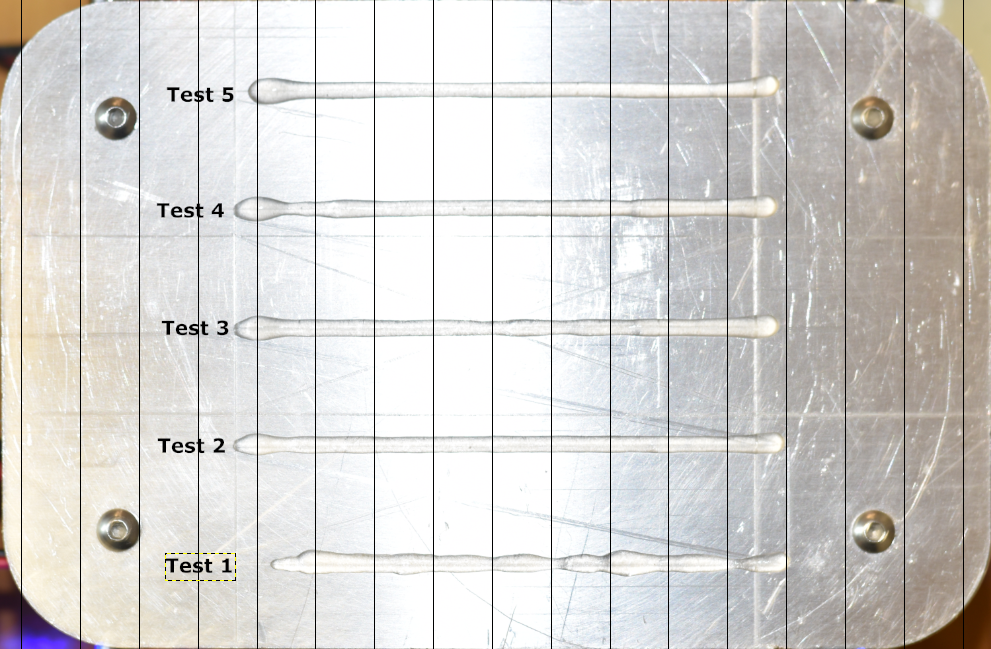
\includegraphics[width=0.6\textwidth]{figs/Phase_1.png}
    \caption{Trial 1 — nozzle height test}
    \label{fig:phase1}
\end{figure}

\begin{figure}[H]
    \centering
    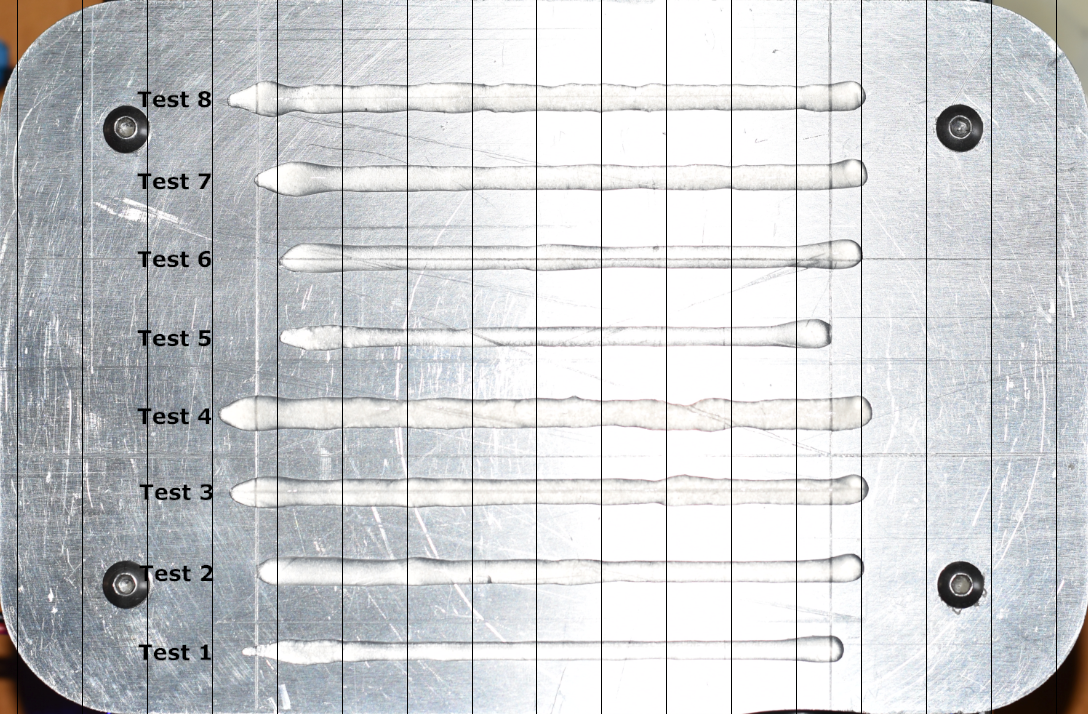
\includegraphics[width=0.6\textwidth]{figs/Phase_2a.png}
    \caption{Trial 2a — straight line test}
    \label{fig:phase2a}
\end{figure}

\begin{figure}[H]
    \centering
    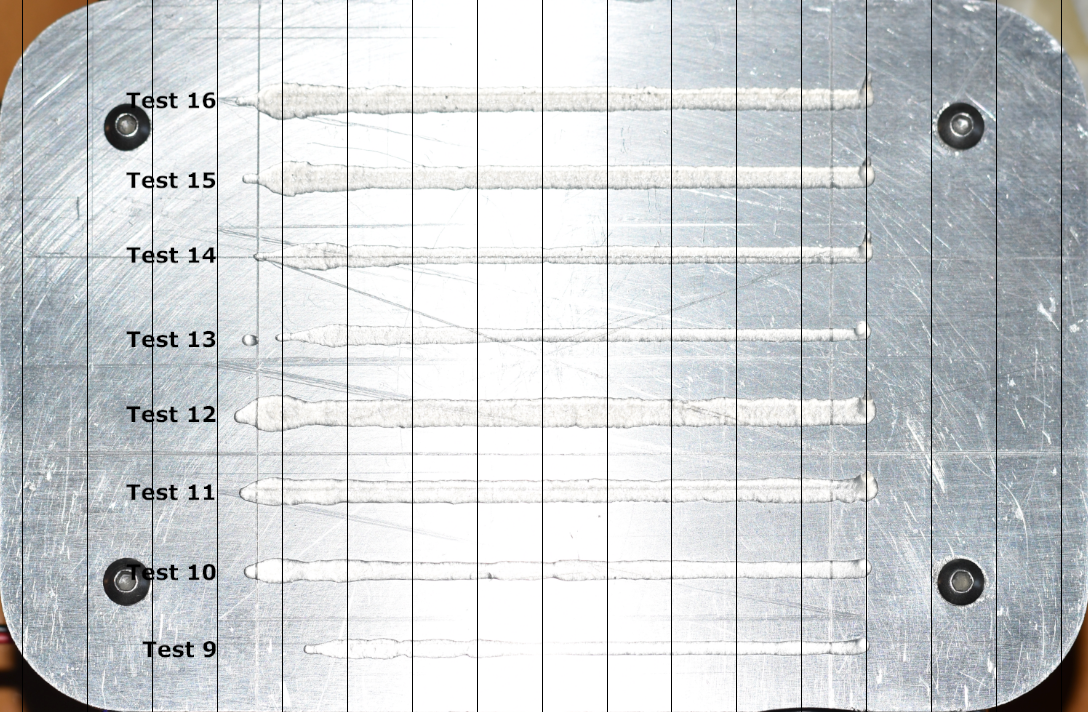
\includegraphics[width=0.6\textwidth]{figs/Phase_2b.png}
    \caption{Trial 2b — straight line test}
    \label{fig:phase2b}
\end{figure}

\begin{figure}[H]
    \centering
    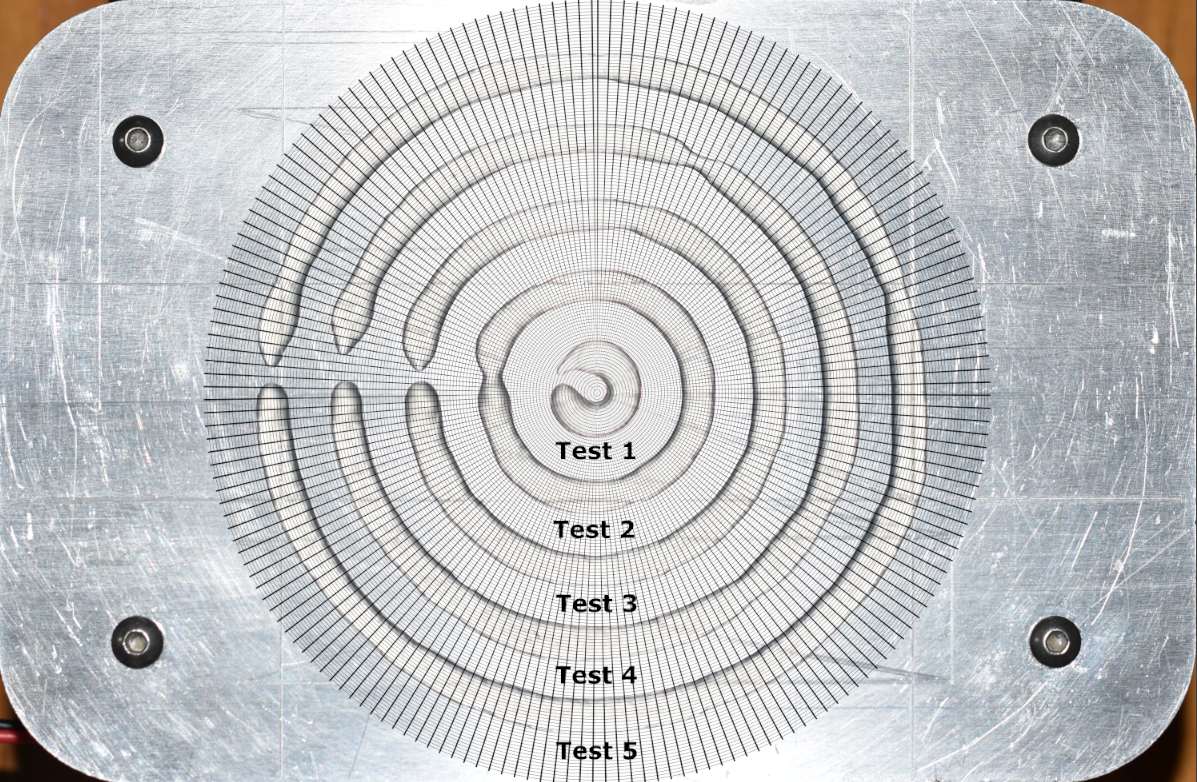
\includegraphics[width=0.6\textwidth]{figs/Phase_3.png}
    \caption{Trial 3 — circle test}
    \label{fig:phase3}
\end{figure}

\begin{figure}[H]
    \centering
    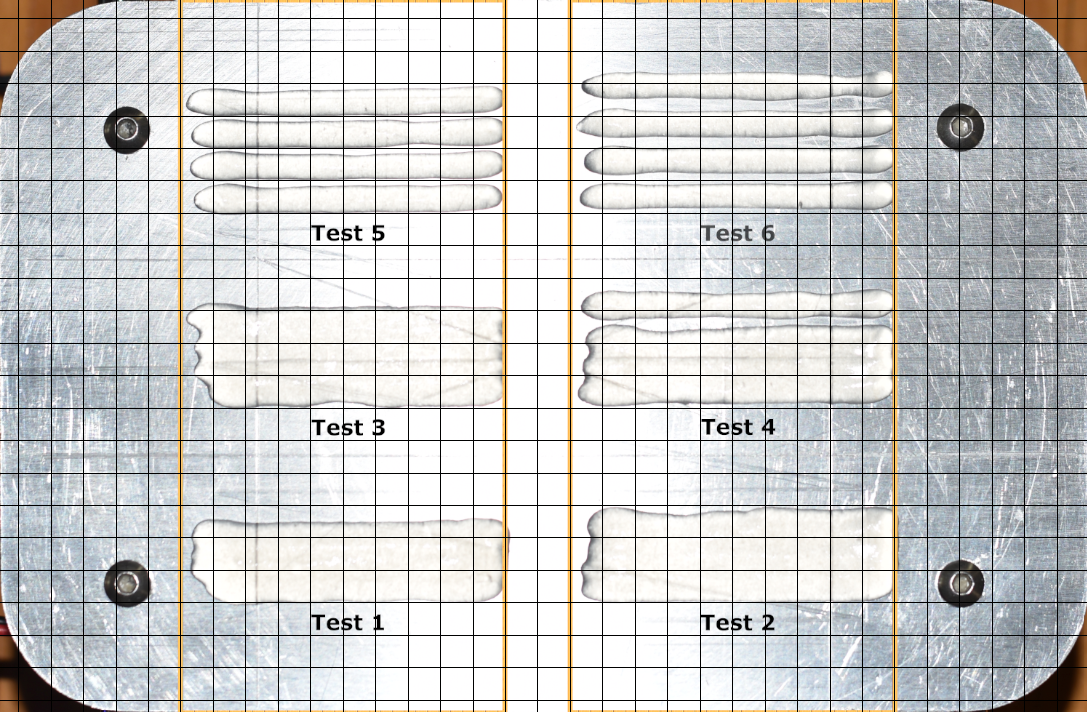
\includegraphics[width=0.6\textwidth]{figs/Phase_4.png}
    \caption{Trial 4 — adjacent lines test}
    \label{fig:phase4}
\end{figure}

\begin{figure}[H]
    \centering
    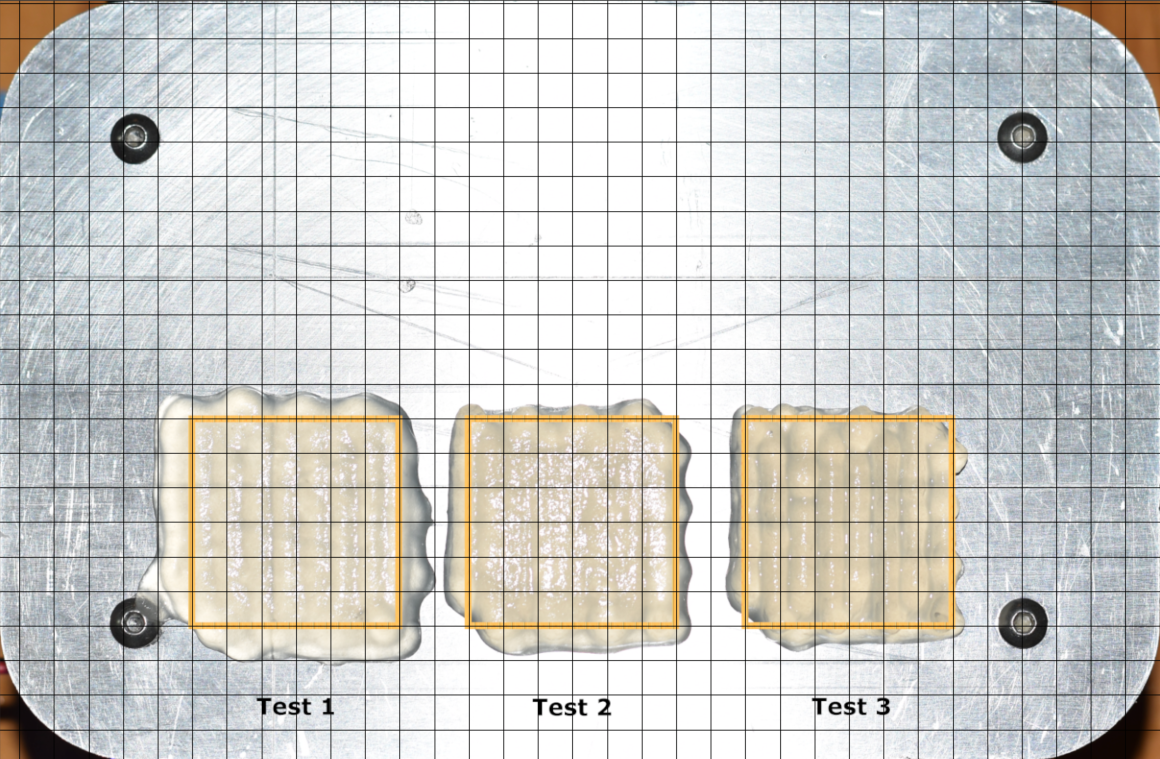
\includegraphics[width=0.6\textwidth]{figs/Phase_5a.png}
    \caption{Trial 5 — stacked layer test}
    \label{fig:phase5a}
\end{figure}
\begin{figure}[H]
    \centering
    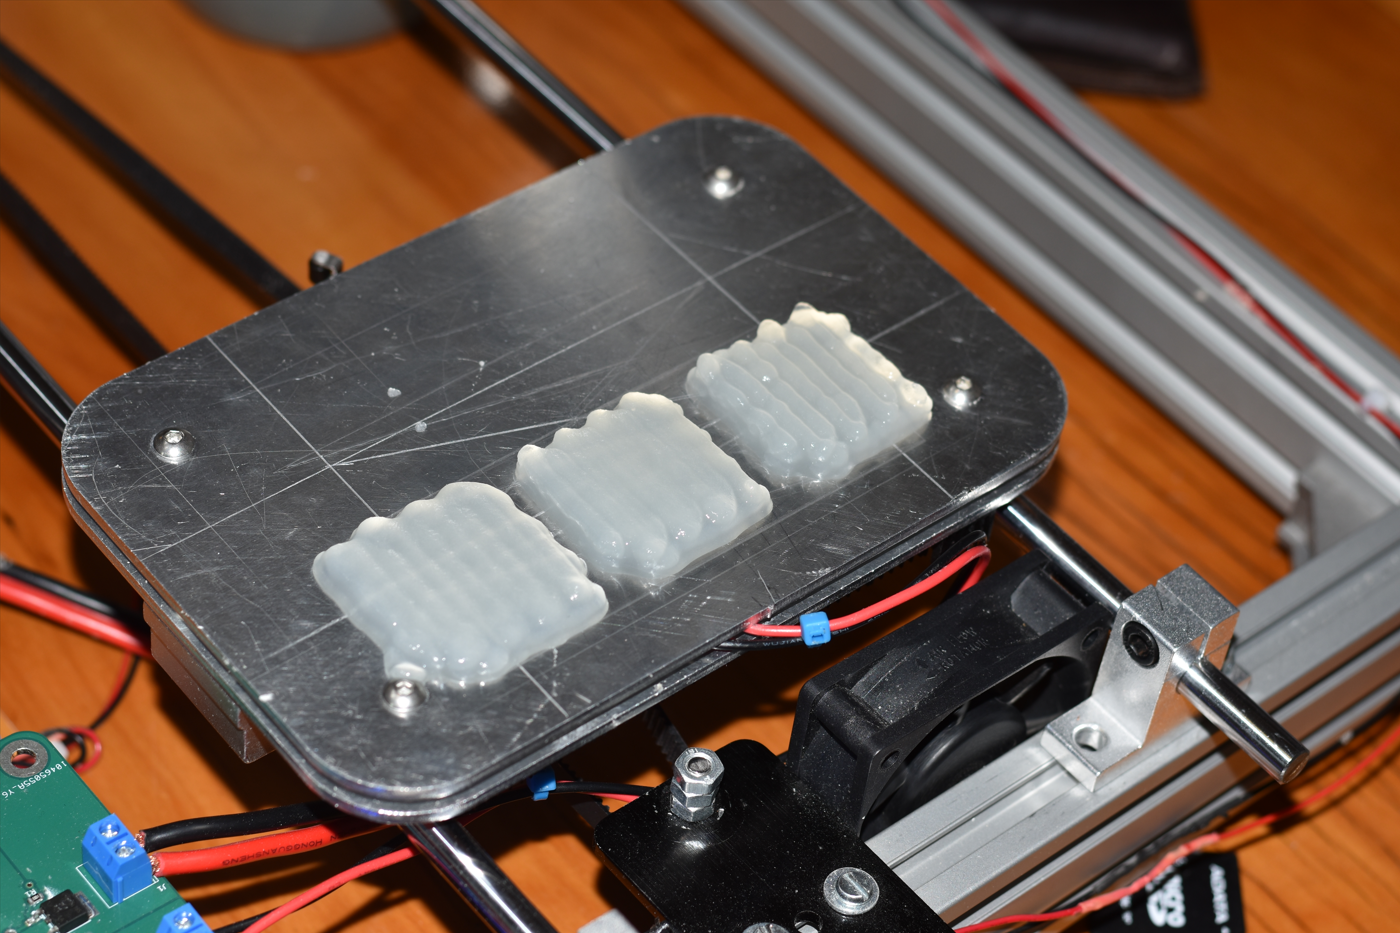
\includegraphics[width=0.6\textwidth]{figs/Phase_5b.png}
    \caption{Trial 5 — angled view}
    \label{fig:phase5b}
\end{figure}

\begin{figure}[H]
    \centering
    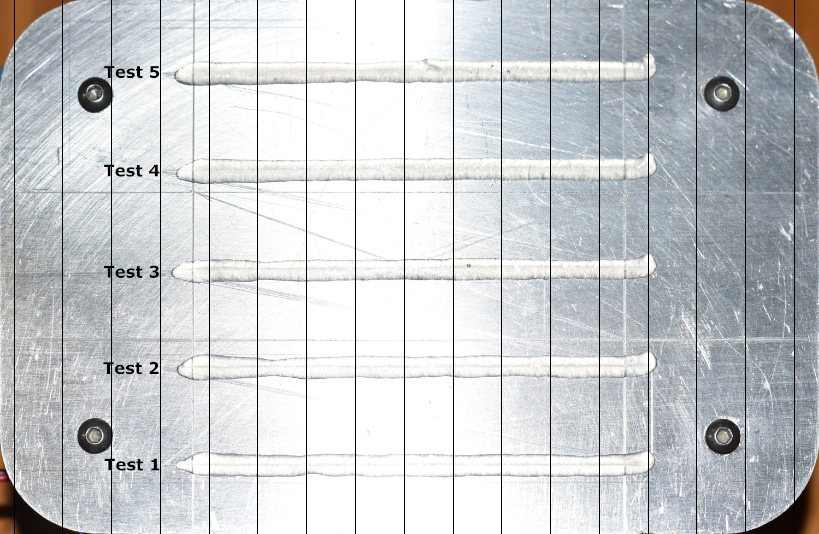
\includegraphics[width=0.6\textwidth]{figs/Phase_6.png}
    \caption{Trial 6 — repeatability test}
    \label{fig:phase6}
\end{figure}